% compile with: pdflatex -shell-escape filename.tex
\documentclass[crop,tikz,convert=pdf2svg]{standalone}
\usepackage{xcolor}
\usetikzlibrary{matrix}

% color list kudos https://sashamaps.net/docs/resources/20-colors/
\definecolor{color1}{HTML}{e6194b}
\definecolor{color2}{HTML}{3cb44b}
\definecolor{color3}{HTML}{ffe119}
\definecolor{color4}{HTML}{4363d8}
\definecolor{color5}{HTML}{f58231}
\definecolor{color6}{HTML}{911eb4}
\definecolor{color7}{HTML}{42d4f4}
\definecolor{color8}{HTML}{f032e6}
\definecolor{color9}{HTML}{bfef45}
\definecolor{color10}{HTML}{fabed4}
\definecolor{color11}{HTML}{469990}
\definecolor{color12}{HTML}{dcbeff}
\definecolor{color13}{HTML}{9a6324}
\definecolor{color14}{HTML}{000075}
\definecolor{color15}{HTML}{800000}
\definecolor{color16}{HTML}{aaffc3}
\definecolor{color17}{HTML}{808000}

\tikzstyle{node}=[
	circle,
  draw,
  fill,
	minimum size=0.75cm,
  text=white,
	thick,
]

\tikzstyle{style1}=[ draw=color1, fill=color1, text=white ]
\tikzstyle{style2}=[ draw=color2, fill=color2, text=white ]
\tikzstyle{style3}=[ draw=color3, fill=color3, text=black ]
\tikzstyle{style4}=[ draw=color4, fill=color4, text=white ]
\tikzstyle{style5}=[ draw=color5, fill=color5, text=white ]
\tikzstyle{style6}=[ draw=color6, fill=color6, text=white ]
\tikzstyle{style7}=[ draw=color7, fill=color7, text=black ]
\tikzstyle{style8}=[ draw=color8, fill=color8, text=white ]
\tikzstyle{style9}=[ draw=color9, fill=color9, text=black ]
\tikzstyle{style10}=[ draw=color10, fill=color10, text=black ]
\tikzstyle{style11}=[ draw=color11, fill=color11, text=white ]
\tikzstyle{style12}=[ draw=color12, fill=color12, text=black ]
\tikzstyle{style13}=[ draw=color13, fill=color13, text=white ]
\tikzstyle{style14}=[ draw=color14, fill=color14, text=white ]
\tikzstyle{style15}=[ draw=color15, fill=color15, text=white ]
\tikzstyle{style16}=[ draw=color16, fill=color16, text=black ]
\tikzstyle{style17}=[ draw=color17, fill=color17, text=white ]

\tikzstyle{heavy edge}=[
	very thick,
]

\tikzstyle{light edge}=[
	very thin,
]

\begin{document}

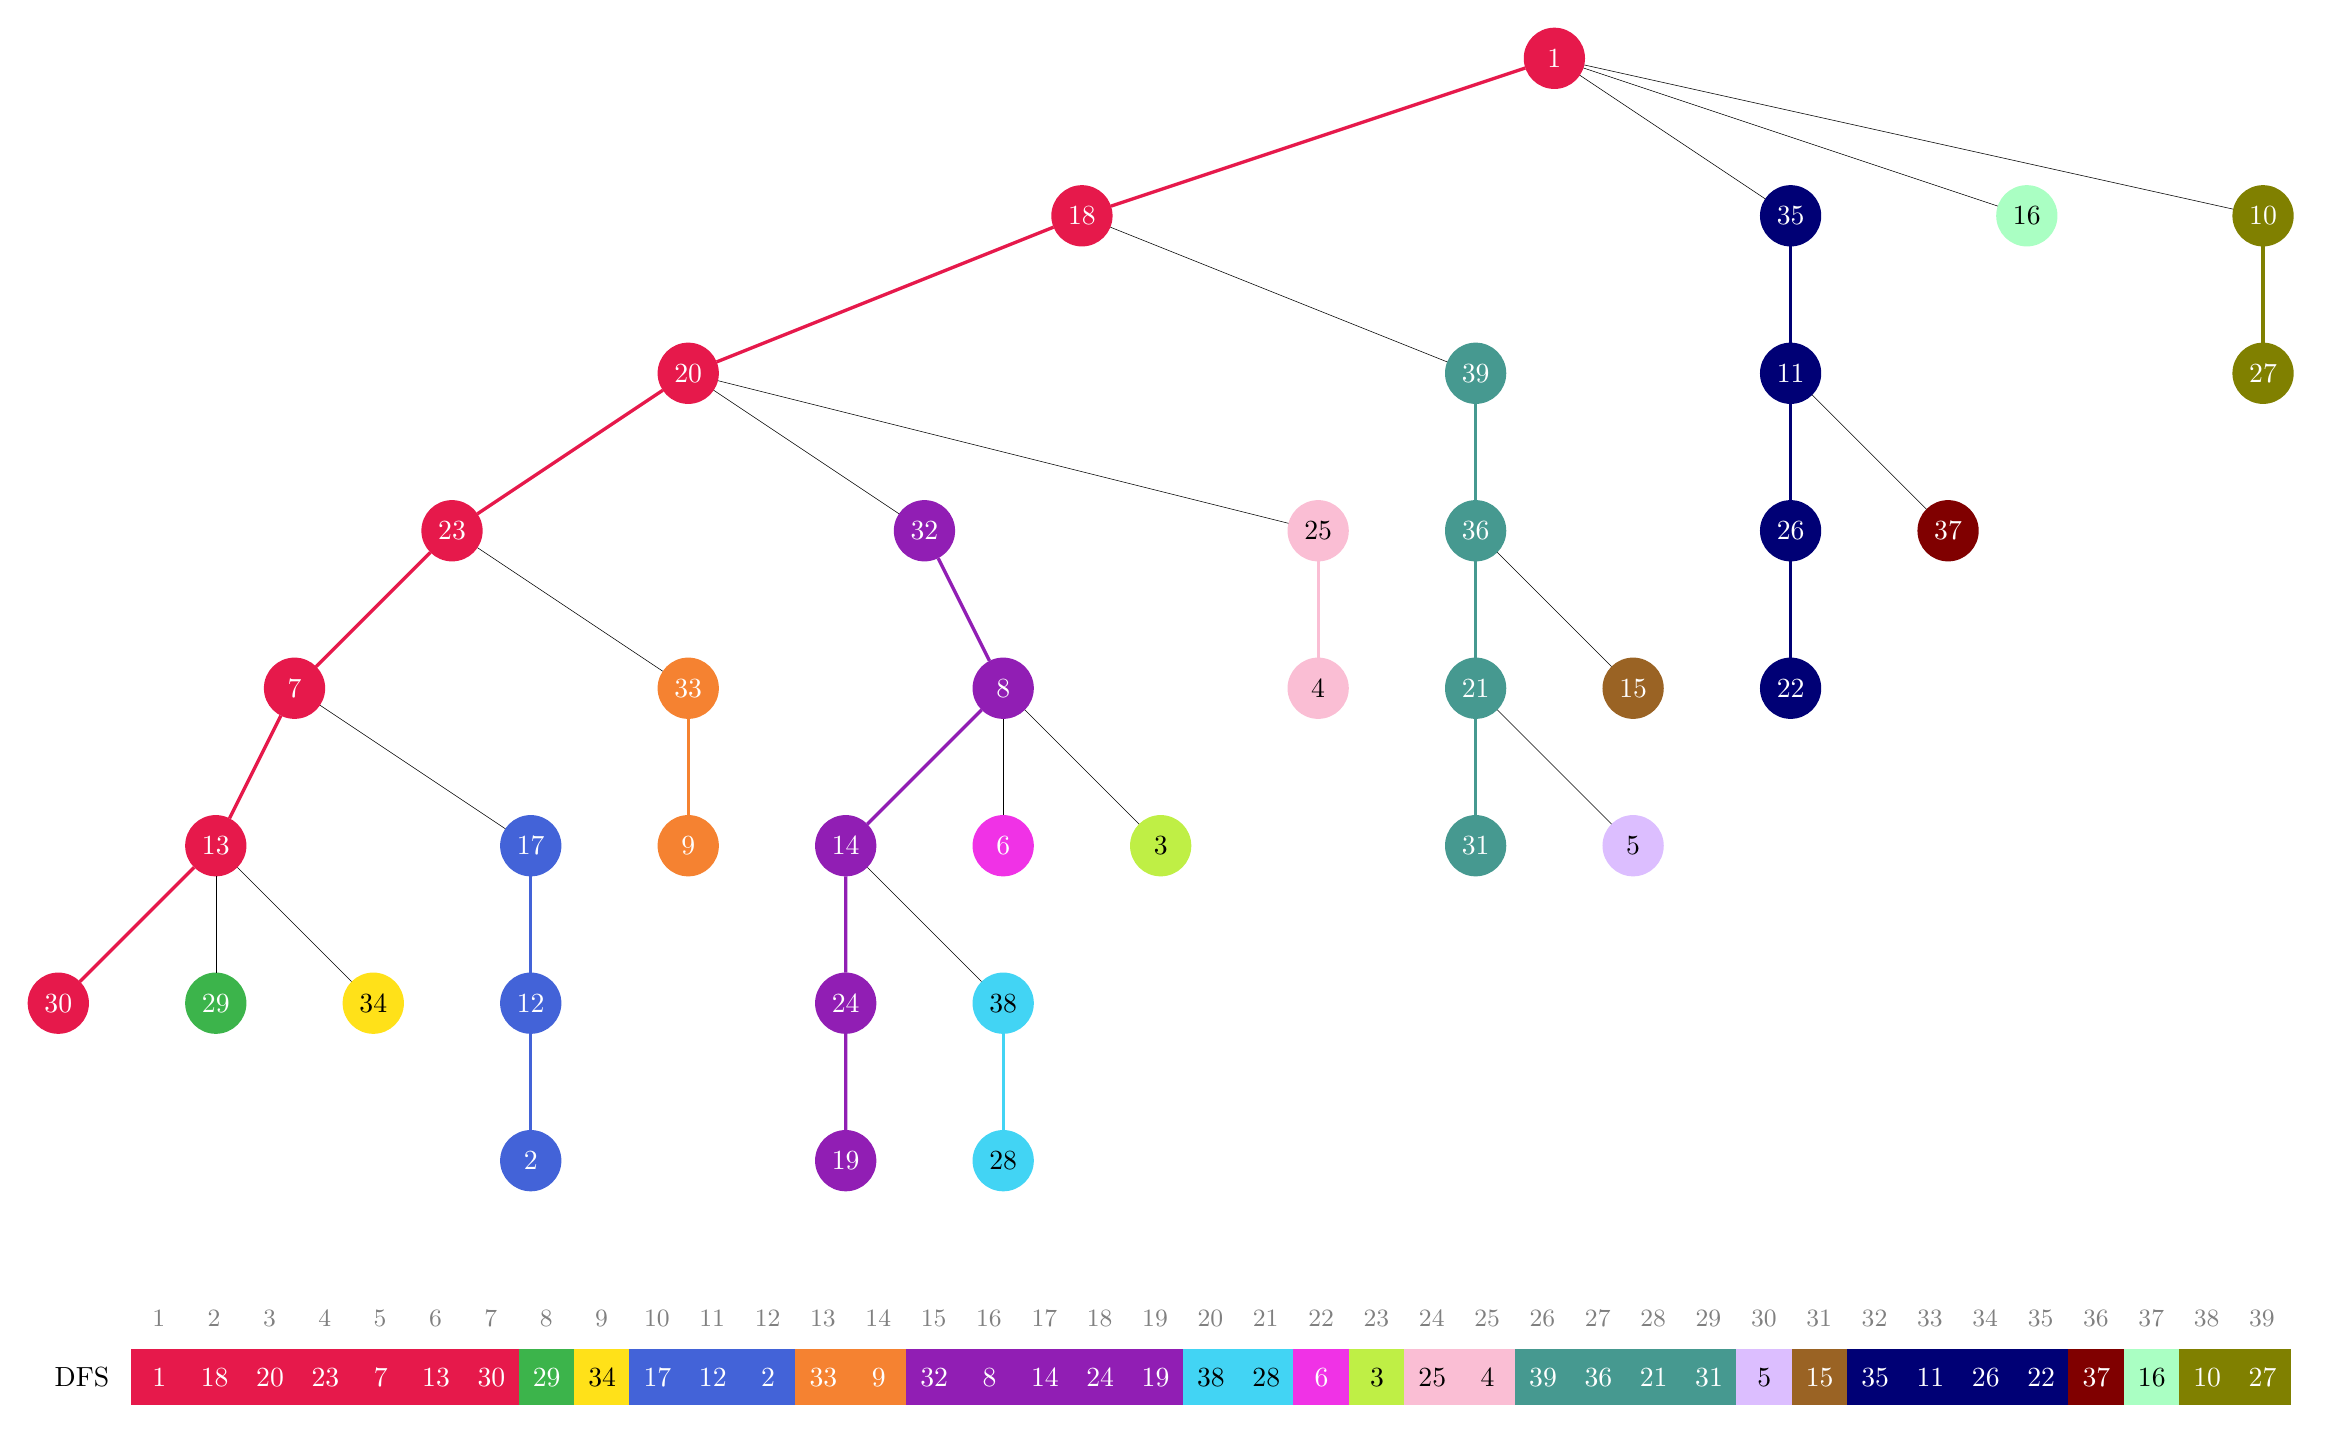
\begin{tikzpicture}
  \node[node, style1] (n1) at (19,0) {$1$};
  \node[node, style1] (n18) at (13,-2) {$18$};
  \node[node, style1] (n20) at (8,-4) {$20$};
  \node[node, style1] (n23) at (5,-6) {$23$};
  \node[node, style1] (n7) at (3,-8) {$7$};
  \node[node, style1] (n13) at (2,-10) {$13$};
  \node[node, style1] (n30) at (0,-12) {$30$};
  \draw[heavy edge, style1] (n1) -- (n18) -- (n20) -- (n23) -- (n7) -- (n13) -- (n30);

  \node[node, style2] (n29) at (2,-12) {$29$};
  \draw[light edge] (n13) -- (n29);

  \node[node, style3] (n34) at (4,-12) {$34$};
  \draw[light edge] (n13) -- (n34);

  \node[node, style4] (n17) at (6,-10) {$17$};
  \node[node, style4] (n12) at (6,-12) {$12$};
  \node[node, style4] (n2) at (6,-14) {$2$};
  \draw[light edge] (n7) -- (n17);
  \draw[heavy edge, style4] (n17) -- (n12) -- (n2);

  \node[node, style5] (n33) at (8,-8) {$33$};
  \node[node, style5] (n9) at (8,-10) {$9$};
  \draw[light edge] (n23) -- (n33);
  \draw[heavy edge, style5] (n33) -- (n9);

  \node[node, style6] (n32) at (11, -6) {$32$};
  \node[node, style6] (n8) at (12,-8) {$8$};
  \node[node, style6] (n14) at (10,-10) {$14$};
  \node[node, style6] (n24) at (10,-12) {$24$};
  \node[node, style6] (n19) at (10,-14) {$19$};
  \draw[light edge] (n20) -- (n32);
  \draw[heavy edge, style6] (n32) -- (n8) -- (n14) -- (n24) -- (n19);

  \node[node, style7] (n38) at (12,-12) {$38$};
  \node[node, style7] (n28) at (12,-14) {$28$};
  \draw[light edge] (n14) -- (n38);
  \draw[heavy edge, style7] (n38) -- (n28);

  \node[node, style8] (n6) at (12,-10) {$6$};
  \draw[light edge] (n8) -- (n6);

  \node[node, style9] (n3) at (14,-10) {$3$};
  \draw[light edge] (n8) -- (n3);

  \node[node, style10] (n25) at (16,-6) {$25$};
  \node[node, style10] (n4) at (16,-8) {$4$};
  \draw[light edge] (n20) -- (n25);
  \draw[heavy edge, style10] (n25) -- (n4);

  \node[node, style11] (n39) at (18,-4) {$39$};
  \node[node, style11] (n36) at (18,-6) {$36$};
  \node[node, style11] (n21) at (18,-8) {$21$};
  \node[node, style11] (n31) at (18,-10) {$31$};
  \draw[light edge] (n18) -- (n39);
  \draw[heavy edge, style11] (n39) -- (n36) -- (n21) -- (n31);

  \node[node, style12] (n5) at (20,-10) {$5$};
  \draw[light edge] (n21) -- (n5);

  \node[node, style13] (n15) at (20,-8) {$15$};
  \draw[light edge] (n36) -- (n15);

  \node[node, style14] (n35) at (22,-2) {$35$};
  \node[node, style14] (n11) at (22,-4) {$11$};
  \node[node, style14] (n26) at (22,-6) {$26$};
  \node[node, style14] (n22) at (22,-8) {$22$};
  \draw[light edge] (n1) -- (n35);
  \draw[heavy edge, style14] (n35) -- (n11) -- (n26) -- (n22);

  \node[node, style15] (n37) at (24,-6) {$37$};
  \draw[light edge] (n11) -- (n37);

  \node[node, style16] (n16) at (25,-2) {$16$};
  \draw[light edge] (n1) -- (n16);

  \node[node, style17] (n10) at (28,-2) {$10$};
  \node[node, style17] (n27) at (28,-4) {$27$};
  \draw[light edge] (n1) -- (n10);
  \draw[heavy edge, style17] (n10) -- (n27);

  \begin{scope}[shift={(0.8,-16)}]
    % First row: indices
    \matrix[right] (index) at (0, 0) [
      matrix of nodes,
      nodes={anchor=center, minimum size=20pt, color=black!50, font=\small},
    ] {
      1 & 2 & 3 & 4 & 5 & 6 & 7 & 8 & 9 & 10 & 11 & 12 & 13 &
      14 & 15 & 16 & 17 & 18 & 19 & 20 & 21 & 22 & 23 & 24 & 25 & 26 &
      27 & 28 & 29 & 30 & 31 & 32 & 33 & 34 & 35 & 36 & 37 & 38 & 39\\
    };

    % Second row: DFS linearization
    \node at (-0.5, -0.75) {DFS};

    \matrix[right] at (0, -0.75) [
      matrix of nodes,
      nodes={draw, anchor=center, minimum size=20pt},
      column sep=-\pgflinewidth,
      row sep=-\pgflinewidth
    ] {
      \node[style1]{1}; &
      \node[style1]{18}; &
      \node[style1]{20}; &
      \node[style1]{23}; &
      \node[style1]{7}; &
      \node[style1]{13}; &
      \node[style1]{30}; &
      \node[style2]{29}; &
      \node[style3]{34}; &
      \node[style4]{17}; &
      \node[style4]{12}; &
      \node[style4]{2}; &
      \node[style5]{33}; &
      \node[style5]{9}; &
      \node[style6]{32}; &
      \node[style6]{8}; &
      \node[style6]{14}; &
      \node[style6]{24}; &
      \node[style6]{19}; &
      \node[style7]{38}; &
      \node[style7]{28}; &
      \node[style8]{6}; &
      \node[style9]{3}; &
      \node[style10]{25}; &
      \node[style10]{4}; &
      \node[style11]{39}; &
      \node[style11]{36}; &
      \node[style11]{21}; &
      \node[style11]{31}; &
      \node[style12]{5}; &
      \node[style13]{15}; &
      \node[style14]{35}; &
      \node[style14]{11}; &
      \node[style14]{26}; &
      \node[style14]{22}; &
      \node[style15]{37}; &
      \node[style16]{16}; &
      \node[style17]{10}; &
      \node[style17]{27}; \\
    };
  \end{scope}

\end{tikzpicture}

\end{document}
